\documentclass[PICOReport.tex]{subfiles}

\begin{document}

%To cover: Galaxy Formation, Clusters, Reionization, point sources (probably moves to a new section called 'Legacy Science')
\subsubsection{The Formation of the First Luminous Sources} 
\label{luminoussources}  
A few hundred million years after the Big Bang, the neutral hydrogen gas permeating the Universe was reionized by photons emitted by the first luminous sources to have formed.  The nature of these sources and the exact history of this epoch are key missing links in our understanding of structure formation (SO5).  
\begin{figure}
\hspace{-0.2in}
\parbox{3.1in}{\centerline {
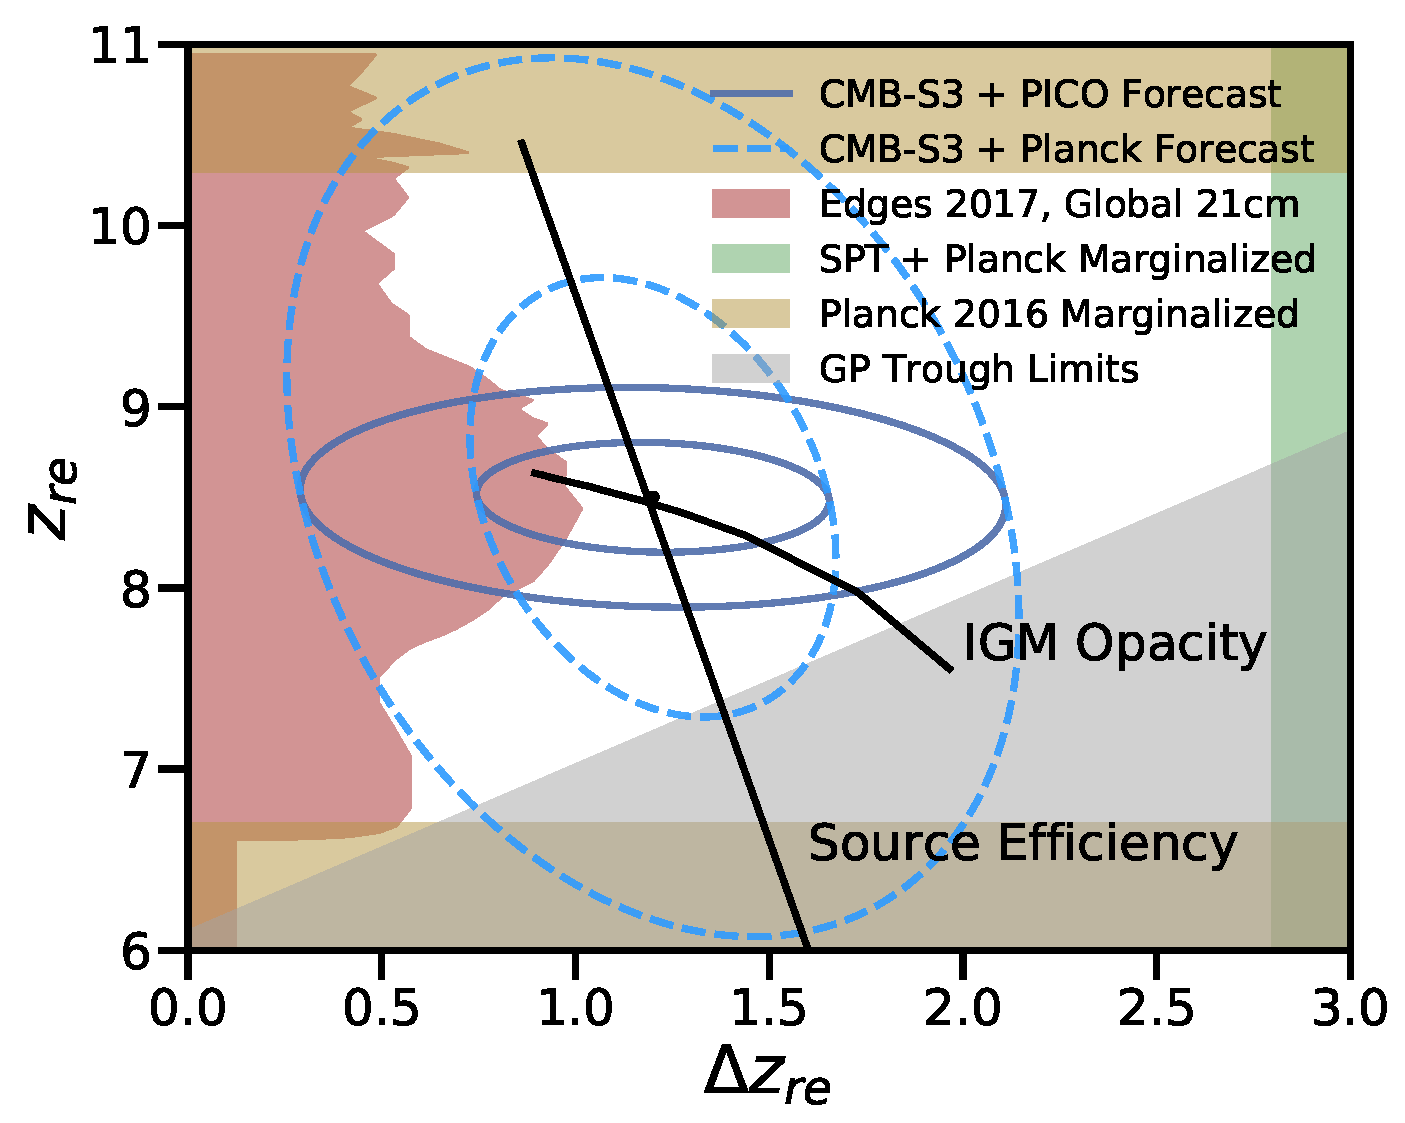
\includegraphics[width=3.0in]{images/Reionization_Contours_zbar_delz_PICO_NEW.pdf} } }
\hspace{0.in}
\parbox{3.5in}{
\caption{\captiontext 
Contours of 1 and 2$\sigma$ constraints on the mean redshift and duration of reionization using PICO and CMB-S3 data (solid dark blue), and comparison with \planck\ and CMB-S3~(dash light blue). Source efficiency and IGM opacity (dark lines) are two physical parameters controlling the reionization process in current models. The PICO measurements, together with higher resolution data of the kSZ effect, will significantly constrain the range of models allowed. We also include other constraints from \planck , EDGES, the Gunn-Peterson (GP) trough, and \planck + the South Pole Telescope~\citep{Planck2018_VI,EDGES2017,Fan2006,Planck2016_reion}.  
\label{fig:ReionizationPICO}
} }
\vspace{-0.1in}
\end{figure}

The reionization of the Universe imprints multiple signals in the temperature and polarization of the CMB.  In polarization, the most important signature is an enhancement in the $EE$ power spectrum at large angular scales $\ell \simlt 10$ (Fig.~\ref{fig:clbb}). This signal gives a direct measurement of the optical depth to the reionization epoch $\tau$ and thus to the mean redshift of reionization $z_{re}$, with very little degeneracy with other cosmological parameters (Fig.~\ref{fig:ReionizationPICO}).\footnote{The mean redshift to reionization is the redshift when $50$\% of the cosmic volume was reionized.} \planck 's determination of the optical depth to reionization $\tau = 0.054 \pm 0.007\, (1\sigma) $ has indicated that reionization concluded by $z \approx 6$, but the measurement uncertainty leaves many unanswered questions including: were the ionizing sources primarily star-forming galaxies or more exotic sources such as supermassive black holes or annihilating dark matter? What was the mean free path of ionizing photons during this epoch?  What was the efficiency with which such photons were produced by ionizing sources?  
%What were the masses and environments of the dark matter halos that hosted the sources?  
Did the reionization epoch extend to $z \approx 15$-$20$, as has been claimed recently?~\citep{Miranda2017} PICO's cosmic-variance-limited measurement of the large-scale $E$ modes reaching $\sigma(\tau)=0.002$ will settle some of these questions and will significantly constrain the others.

Figure~\ref{fig:ReionizationPICO} presents forecasts for reionization constraints in the $z_{re} - \Delta z_{re}$ parameter space. These are obtained from PICO's measurement of $\tau$ in combination with S3 experiments measurements of the ``patchy'' kinematic Sunyaev-Zel$^{\prime}$dovich (kSZ) effect, due to the peculiar velocities of free electron bubbles around ionizing sources~\citep{Calabrese2014}.
The figure includes curves of constant efficiency of production of ionizing photons in the sources, and of intergalactic-medium opacity, two parameters that quantify models of reionization. The curves shown are illustrative; families of models, that would be represented by parallel \lq source efficiency\rq~and \lq IGM Opacity\rq~lines, are allowed by current data. PICO's data will give simultaneous constraints on these physical parameters, yielding important information on the nature of the first luminous sources. For example, galaxies and quasars predict significantly different values for their IGM opacities and source efficiencies.  


The process of reionization leaves specific non-Gaussian signatures in the CMB.  In particular, patchy reionization induces non-trivial 4-point functions in both temperature and polarization~\citep{SmithFerraro2017,DvorkinSmith2009}.  The temperature 4-point function can be used to separate reionization and late-time kSZ contributions.  Combinations of temperature and polarization data can be used to build quadratic estimators for reconstruction of the patchy $\tau$ field, analogous to CMB lensing reconstruction (next Section).  These estimators generally require high angular resolution, but also rely on foreground-cleaned CMB maps.  PICO's data in its high-frequency bands --- which have better than 2~arcmin resolution and cover frequencies that are not suitable for observations from the ground --- will enable these estimators to be robustly applied to high resolution ground-based CMB data, a strong example of ground-space complementarity.  %\comor{if pico is complementarity by {\it only} providing foreground maps at sufficiently high resolution, I think we should move this to the 'complementarity'. It is not a direct science goal or outcome.}
%% JCH: I checked the Smith-Ferraro 4-pt estimator, and PICO does not have sufficient resolution to do this (see Fig. 3 of https://arxiv.org/pdf/1803.07036.pdf )
%
%Thus, while PICO alone may not enable high \ac{SNR} reconstructions,

With ten independent maps of the entire sky, multiple frequency bands and ample sensitivity to remove foregrounds, PICO is uniquely suited to make the low $\ell$ $EE$-spectrum measurements that are needed to elucidate the formation of the first luminous sources. No such measurements have yet been done from the ground. Of the currently operating and planned S3 experiments, one is targeting the lowest $\ell$ $EE$ spectrum~\citep{class_overview}. 

Lowering the uncertainty on $\tau$ is crucial for many cosmological observables of the growth of structure. As discussed in Section~\ref{neutrino_fundamental}, these observables require knowledge of the amplitude of the initial fluctuations power spectrum $A_s$; however, the signatures of $A_{s}$ and $\tau$ are degenerate in the %primary
CMB power spectra, except in the low-$\ell$ $EE$ power spectrum.  PICO's cosmic-variance-limited polarization measurements will break this degeneracy and thus improve constraints on the sum of neutrino masses, on dark energy, and modified gravity coming from {\it any} low-z growth measurement such as CMB and galaxy lensing, velocity-field measurements, redshift-space distortions, and galaxy surveys. 

%%%%%%%%%%
\subsubsection{Probing the Evolution of Structures via Gravitational Lensing and Cluster Counts} 
\label{sec:gravitationallensing}

The particle content of the Universe, gravitational collapse, the effects of dark energy, and energetic feedback processes that recycle energy determine the evolution of structures in the Universe. The amplitude of linear fluctuations as a function of redshift, parameterized through $\sigma_8(z)$, is thus a sensitive probe representing the effects of physical process affecting growth. \ac{CMB} photons are affected by, and thus probe $\sigma_{8}(z)$ as they traverse the entire Universe. PICO will tightly constrain $\sigma_8(z)$ through measurements of gravitational lensing and cluster counts. 

\noindent$\bullet$ {\bf Gravitational Lensing} \hspace{0.1in} \label{lensing} Matter between us and the last-scattering surface deflects the path of photons through gravitational lensing, imprinting the 3-dimensional matter distribution across the volume of the Universe onto the CMB maps. The specific quantity being mapped by the data is the projected gravitational potential $\phi$ that is lensing the photons. From the lensing map, which receives contributions from all redshifts between us and the CMB, with the peak of the distribution at $z \simeq 2$, we infer the angular power spectrum $C_{L}^{\phi \phi}$ (Fig.~\ref{fig:lensingNoisePICO}). Both the temperature and polarization maps of the CMB, and by extension the angular power spectra, are affected by lensing. 
\begin{figure}[h]
\hspace{-0.2in}
\parbox{3.0in}{\centerline {
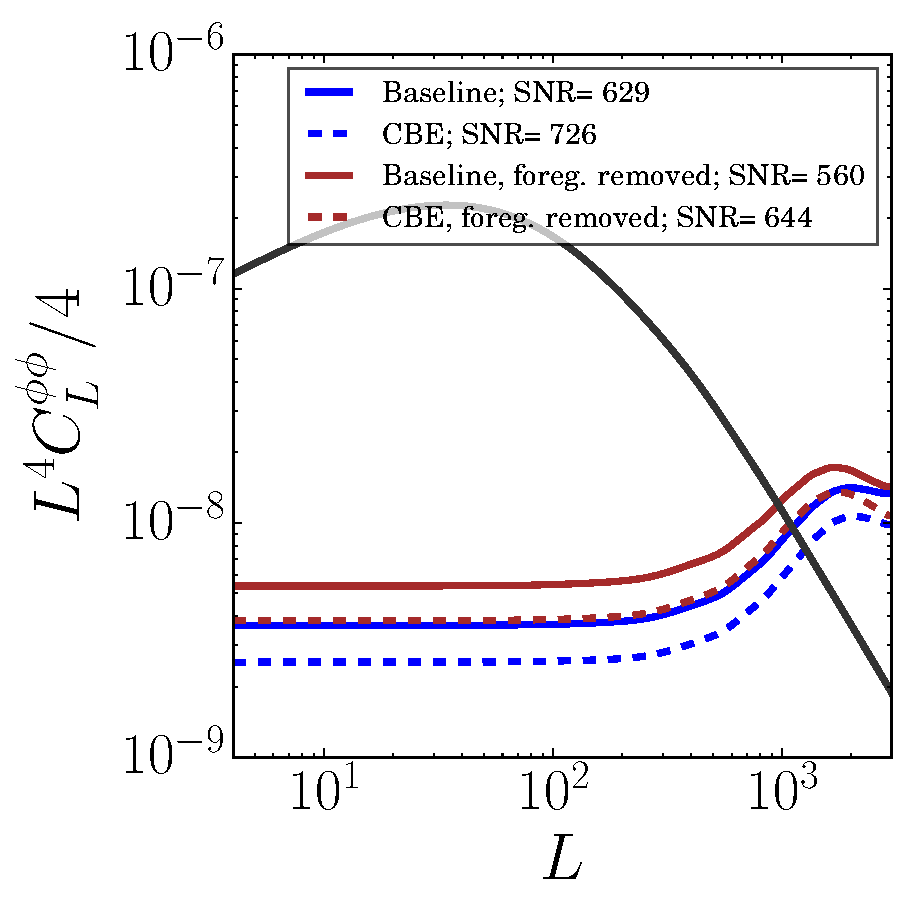
\includegraphics[width=2.2in]{images/lensingNoisePICO.pdf} } }
\hspace{0.in}
\parbox{3.3in}{
\caption{\captiontext 
PICO will make a high \ac{SNR} full sky map of the projected gravitational potential $\phi$ due to all matter between us and the last scattering surface at all angular scales $L$ for which its noise (red and blue) is below the 
theoretically predicted power spectrum $C_{L}^{\phi \phi}$ (black). Noise predictions are given with (dash) and without (solid) foregrounds separation, and we include values for the \ac{SNR} for the measurement of $C_{L}^{\phi \phi}$ for 
$2 \leq L \leq 1000$. 
%The map of $\phi$ will be made using a map of $B$-mode arising from the gravitational lensing of \ac{CMB} photons by the large scale structure of the Universe. 
\label{fig:lensingNoisePICO} 
} }
\vspace{-0.1in}
\end{figure}

\planck 's $\phi$ map had \ac{SNR} of $\sim$1 per $L$ mode over a narrow range of scales, $30 < L < 50$.\footnote{$L$ refers to multipoles in the CMB lensing and galaxy clustering fields, in contrast to the use of $\ell$  for the CMB itself. } PICO's map would represent true mapping, with \ac{SNR} $\gg1$ for each mode in the range $2 \leq L \lesssim 1000$.  While \planck\ had an \ac{SNR} of 40 integrated across the entire $C_{L}^{\phi \phi}$ power spectrum~\citep{2018arXiv180706210P}, PICO will give \ac{SNR} of 560 and 644 for the baseline and CBE configurations, respectively; both values already account for foreground separation (Fig.~\ref{fig:lensingNoisePICO}). 

PICO's $\phi$ map is a key ingredient in the delensing process that improves constraints on $r$~(\S~\ref{sec:inflation}) and in extracting neutrino mass constraints~(\S~\ref{sec:relics_neutrinos}). It will also be used to constrain the properties of quasars and other high-redshift astrophysics.  For example, cross-correlations with quasar samples from DESI will yield a precise determination of the quasar bias (and hence host halo mass) as a function of the quasar properties, such as (non-)obscuration.  Such studies are not possible with any other lensing techniques, due to their sensitivity to lower redshifts.

%\comor{Lensing will also be used to weigh dark matter halos hosting galaxies, quasars, and groups and clusters of galaxies.  In the context of quasar analyses described above, this halo mass information is in the ``one-halo'' term of the cross-correlation, while the bias information is in the ``two-halo'' term.  PICO will access both sets of information, allowing consistency tests and further tightening constraints.  Detailed forecasts for halo lensing are presented in the cluster subsection below.}

\noindent$\bullet$ {\bf $\sigma_{8}(z)$ from Gravitational Lensing} \hspace{0.1in} \label{sigma8_lensing}
Cross-correlations between the PICO lensing potential map and wide-field samples of galaxies and quasars provide a powerful technique to measure the time dependence of the amplitude of matter fluctuations $\sigma_{8}(z)$ in tomographic redshift bins. This is achieved by overcoming the limitations of auto-correlations of these data sets:
The lensing $\phi$ map is sensitive to the projection of all matter back to the last scattering surface, so it cannot resolve the time dependence of fluctuations, while galaxies and quasars trace matter in an unknown biased way so that the matter amplitude cannot be determined.
Cross-correlations of the two data sets, broken down to several tomographic redshift bins, will constrain how galaxies in each bin trace the dark matter, which will yield strong constraints on $\sigma_8(z)$ and thereby on structure formation and models of dark energy and modified gravity~\citep{2009PhRvL.102b1302S,2018PhRvD..97l3540S}.

In Fig.~\ref{fig:sigma8} we show projected $1\sigma$ errors on $\sigma_8(z)$ when using cross-correlations with LSST's gold sample of galaxies~\citep{LSSTSciBook}.  Sub-percent accuracy is obtainable with PICO's resolution which will give information extending to $L =1000$.\footnote{PICO's resolution is sufficient to give information for $L>1000$, but at these scales structures are non-linear and will not be used to constrain $\sigma_{8}(z)$.} This accuracy will be used to constrain dark energy or modified gravity, in the context of specific models, and to give a neutrino mass constraint that is independent from and competitive with that inferred from the CMB lensing auto-power spectrum (\S~\ref{neutrino_fundamental})~\citep{2018arXiv180902120Y} .

\begin{figure}
\centering
\hspace{-0.15in}
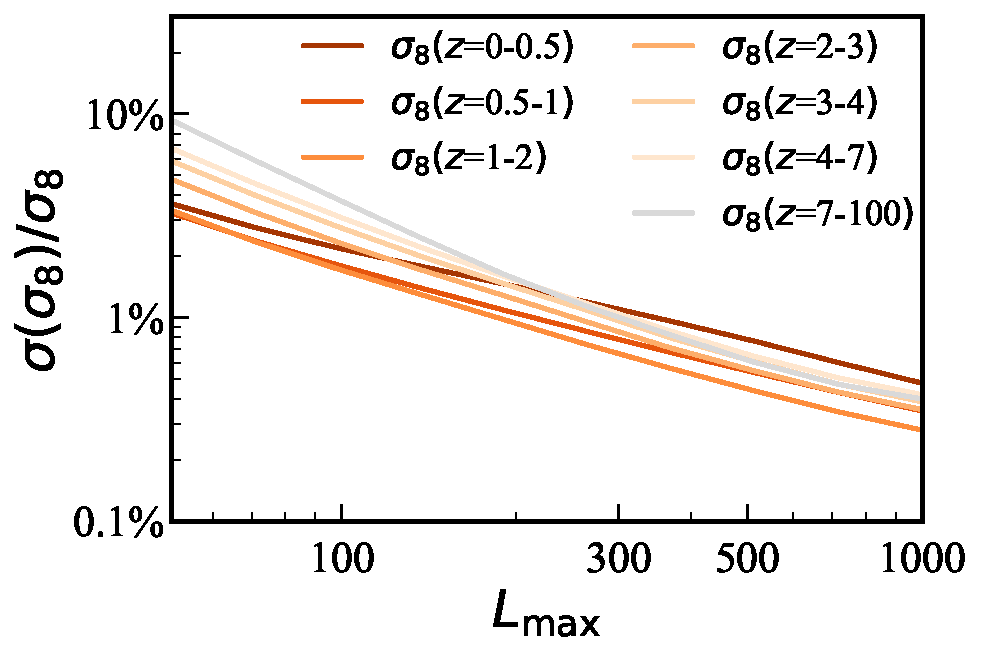
\includegraphics[width=3in]{images/PICO_s8_lmax_PICOv4.1b_deproj0_SENS0_LSST10yrGold.pdf}
\hspace{-0.1in}
\includegraphics[width=2.9in,trim= 0cm 0.2cm 0cm 0cm]{images/PICOS8.png}
\caption{\captiontext  
Sub-percent constraints on the evolution of $\sigma_{8}$ as a function of redshift will come from two independent PICO products: Correlations between PICO's deep gravitational lensing map (Fig.~\ref{fig:lensingNoisePICO}) and LSST's gold sample of galaxies (left) and cluster counts (right). Fractional uncertainties in $\sigma_{8}$ relative to fiducial $\Lambda$CDM values are given as a function the finest angular scale $L_{max}$ of the correlation analysis for seven redshift bins (left).  The baseline and CBE configurations give essentially the same fractional errors of $\sigma_{8}(z)$ using cluster counts (right).  LSST assumptions: 10 years, 50\% sky fraction, 55 galaxies per ${\rm arcmin}^{2}$ at redshift $z<3$ with magnitude limit $i <25.3$~\citep{LSSTSciBook}, and dropout galaxies at $z>3$~\citep{dropouts} extrapolating recent Hyper Suprime-Cam observations~\cite{Schmittfull/Seljak,HSC1,HSC2}, with linear bias $b(z)=1+z$.
\label{fig:sigma8} }
\end{figure}

\noindent$\bullet$ {\bf Cluster Counts} \hspace{0.1in} \label{clusters}  
The distribution of galaxy clusters in redshift is one consequence of the evolution of structures and is thus a sensitive measure of $\sigma_{8}(z)$. The observational quantity of interest is $dN/dz \,\, d m $, the number of observed clusters per redshift and per mean mass, from which constraints on $\sigma_{8}$ can be derived. Galaxy clusters found by PICO via the \ac{tSZ} effect (\S~\ref{sec:sz}) provide a catalog with a selection function that is simple to model and thus straightforward to use for cosmological inference. PICO's catalog will provide all clusters with masses above $\sim3\times10^{14} M_\odot$\footnote{$M_\odot$ is one solar mass} \comor{check values} out to redshifts $z\sim3$, as long as the clusters have started to virialize. We forecast that PICO will find $\sim$150,000 galaxy clusters, assuming the cosmological parameters from \planck\  and using the 70\% of sky not obscured by the Milky Way.  Redshifts will be provided by optical and infrared follow-up surveys.  Cluster masses will be inferred by optical weak lensing for clusters with $z < 1.5$ and by PICO's own CMB halo lensing data at higher redshifts (see discussion of halo lensing below). The catalog will give the most massive clusters over the full sky. Sub-percent determination of $\sigma_{8}$ will be provided with this catalog for $0.5 < z < 2$ (Fig.~\ref{fig:sigma8}), and a neutrino mass constraint of $\sim$10~meV that is independent from the one coming from the lensing measurements (\S~\ref{sec:relics_neutrinos}). 

%\comor{Now to connect to $\sigma_{8}$ quantitatively in the last sentence. Need to compare to SO. Need to explain why this is compelling. Need to explain why PICO (e.g. full sky coverage) probe?}
%\comor{Points to still hit High z sample, Numbers -- Nick and Jim should cross-check, most massive cluster all over the whole sky,
%Cosmology.}

Calibrating the masses of clusters, that is determining $m(z)$, is the most uncertain step in inferring $\sigma_{8}$ and other cosmological parameters using cluster counts.  PICO will provide calibration using `CMB halo lensing', an approach that uses the small-scale effects of gravitational lensing due to dark matter halos around clusters and proto-clusters~\citep{2015ApJ...806..247B, 2015PhRvL.114o1302M, 2016A&A...594A..24P}. The technique is particularly effective for measuring halo masses out to high redshifts where gravitational lensing of background objects no longer works because there are no background sources. 
The approach is illustrated in Fig.~\ref{fig:HaloLensing}, which gives the $1\sigma$ uncertainty in a halo mass measurement as a function of the object's redshift. PICO will measure the mass of individual low-mass clusters ($\sim 10^{14}$\,M$_\odot$) over a wide redshift range, and by stacking will determine the mean mass of smaller halos, with masses of $\sim 10^{13}$\,M$_\odot$, which include those hosting individual galaxies. Because the vast majority of clusters have masses that are larger than $\sim 10^{14}$\,M$_\odot$, the PICO data will provide mass calibration for all objects of interest. The flattening at high redshift reflects the fact that the technique is sensitive over a broad range of redshifts. The high-frequency PICO data, at which the resolution matches ground-based instruments' resolution at lower frequencies, will play an essential role in cleaning foregrounds particularly those derived from the temperature-based estimator, which is most contaminated by foregrounds. 
\begin{figure}[h]
\hspace{-0.1in}
\parbox{3.1in}{\centerline {
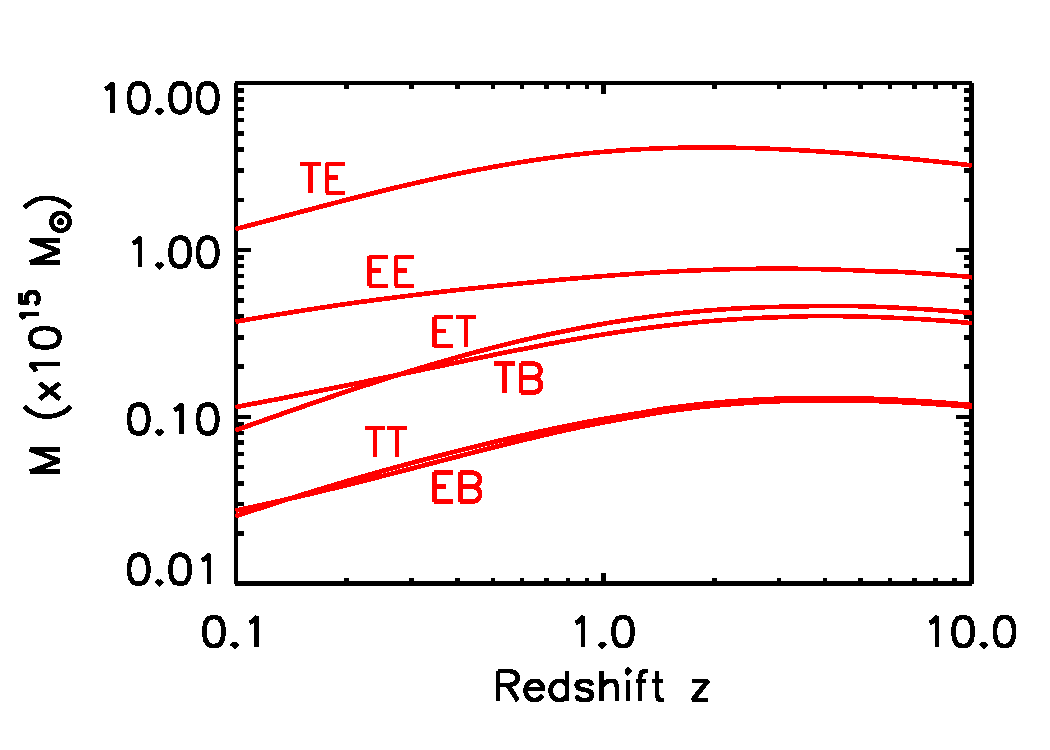
\includegraphics[width=3.0in]{images/m500lim_vs_z_pico_polar_v4.pdf} } }
\hspace{0.in}
\parbox{3.4in}{
\caption{\captiontext 
PICO will provide mass calibration for individual clusters and proto-clusters with mass as low as $10^{14}$ solar masses at $z>2$ using `halo lensing'. Curves for different CMB signal correlations (red) give the $1\sigma$ sensitivity of an optimal mass filter~\citep{2015A&A...578A..21M} for a given mass as a function of $z$.  The curves are flat at high redshift, demonstrating that the technique probes a broad range of red-shifts. For PICO, the $EB$ and $TT$ estimators are equivalent, offering important cross-validation of measurements because the systematics are very different for temperature and polarization. 
\label{fig:HaloLensing} 
} }
\vspace{-0.2in}
\end{figure}

Beyond its role in calibrating masses for cluster counts, PICO's halo lensing measurements will also be a unique tool for measuring the relation between galaxies and their dark matter halos during the key epochs of cosmic star formation at $z\geq 2$, which is not reachable by other means.  This will provide valuable insight into the role of environment on galaxy formation during the rise to and fall from the peak of cosmic star formation at $z\sim 2$. 

%the mass sensitivity of PICO using a spatial filter optimized for extracting the mass of halos \citep{2015A&A...578A..21M}.  The curves give the $1\sigma$ noise in a mass measurement through the filter as a function of redshift. 


\subsubsection{Constraining Feedback Processes through the Sunyaev--Zel$^{\prime}$dovich Effect}
%Compton-$y$ map and tSZ auto-power spectrum} 
\label{sec:sz}
%\label{ymap}  


%\subsubsection{Constraining Structure Growth and Galaxy Formation via the Sunyaev-Zel$^{\prime}$dovich (SZ) Effects} 
% \label{sec:sz}

Not all CMB photons propagate through the Universe freely; about 6\% are Thomson-scattered by free electrons in the \ac{IGM} and \ac{ICM}.  These scattering events leave a measurable imprint on \ac{CMB} temperature fluctuations, which thereby contain a wealth of information about the growth of structures and the thermodynamic history of baryons. A fraction of these photons are responsible for the thermal and kinetic Sunyaev--Zel$^{\prime}$dovich effects (tSZ and kSZ)~\citep{zeldovich69,SZ1972}. The amplitudes of the tSZ and kSZ signals are proportional to the integrated electron pressure and momentum along the line of sight, respectively.  They thus contain information about the thermodynamic properties of the \ac{IGM} and \ac{ICM}, which are highly sensitive to astrophysical feedback. Feedback is the process of energy injection into the \ac{IGM} and \ac{ICM} from accreting supermassive black holes, supernovae, stellar winds, and other sources. Feedback processes are the most uncertain, yet crucial, ingredient in modern theories of galaxy formation; they are required in order to match observations of the stellar properties of galaxies, but the underlying details of the physical processes involved are still highly uncertain.

%%%%%%%%%%%%%%%%%%%%
%\subsubsection{Constraining Feedback Processes: Compton-$y$ map and tSZ auto-power spectrum} 
%\label{ymap}  

Multifrequency \ac{CMB} data also allow the reconstruction of full-sky maps of the tSZ signal, commonly called  \lq Compton-$y$ map\rq. With low noise and broad frequency coverage, which is essential for separating out other signals, PICO will yield a definitive Compton-$y$ map over the full sky, with a total \ac{SNR} of 1270 for the CBE and $\approx 10$\% lower for the baseline configurations (Fig.~\ref{fig:PICO_tSZ_PS}). This is nearly two orders of magnitude higher \ac{SNR} than \planck , which already gave data with much higher \ac{SNR} than ground-based experiments. 
%\comor{how does PICO compare to SO?.}
\begin{figure}[h]
\hspace{-0.1in}
\parbox{3.1in}{\centerline{
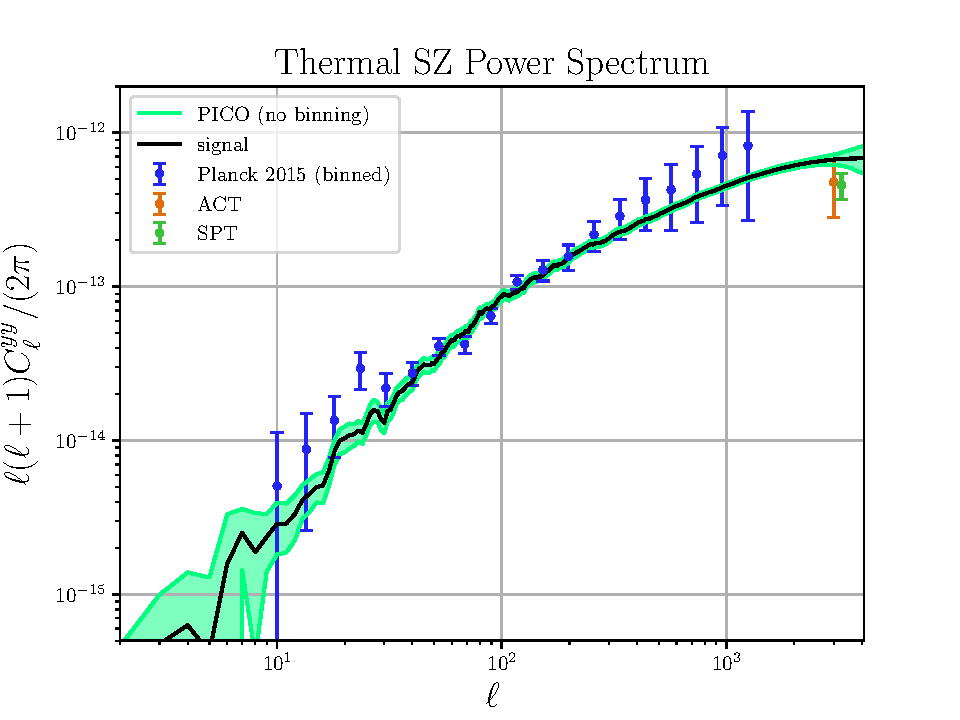
\includegraphics[width=3.0in]{images/PICO_tSZ_PS_plot.pdf} } }
\hspace{0.in}
\parbox{3.4in}{
\caption{\captiontext  
The PICO $y$-map will give a tSZ power spectrum with an \ac{SNR} of 1270 (green, $1\sigma$ per $\ell$ mode), which is nearly 100 times larger than from \planck\ (blue). Binning the data (not shown) as was done for \planck\ would further increase the \ac{SNR}.  We include current measurements by the ground-based SPT and ACT~\citep{Sievers2013,George2015}. In these forecasts we reconstruct the Compton-$y$ field from maps that include Galactic foregrounds, CMB fluctuations, and PICO CBE noise using the needlet internal linear combination algorithm~\citep{Delabrouille2009}. The input maps use the \planck~sky model~\cite{psm?}.
%The black curve shows the simulated tSZ power spectrum signal.  The light green shaded region shows the error bars for PICO at each multipole, i.e., with no binning, as determined from NILC analysis of full-sky simulations.  The blue points show the current constraints from Planck, which have been averaged into broad multipole bins.  The orange and dark green points show the constraints from ACT and SPT, respectively, at a single multipole of $\ell=3000$.  The overall PICO $S/N = 1270$, nearly two orders of magnitude larger than current measurements.
\label{fig:PICO_tSZ_PS} 
} }
\vspace{-0.1in}
\end{figure}

Strong constraints on models of astrophysical feedback will be obtained from the analysis of the PICO $y$-map, both from its auto-power spectrum and from cross-correlations with galaxy, group, cluster, and quasar samples. 
% Like the CMB-lensing map described above, the legacy value of the PICO $y$-map will be immense.  
As an example, we forecast the detection of cross-correlations between the PICO $y$-map and galaxy weak lensing maps constructed from LSST and WFIRST data.  Considering the LSST \lq gold\rq~sample with a source density of 26 galaxies/arcmin${}^2$ covering 40\% of the sky, we forecast a detection of the tSZ-weak lensing cross-correlation with \ac{SNR} = 3000.  Cross-correlations with the galaxies themselves will be measured at even higher \ac{SNR}.  At this immense significance, the signal can be broken down into dozens of tomographic redshift bins, yielding a precise tracing of the evolution of thermal pressure over cosmic time.  For PICO and WFIRST (assuming 45 galaxies/arcmin${}^2$ covering 5.3\% of the sky), we forecast \ac{SNR} = 1100 for the tSZ-weak lensing cross-correlation.  The WFIRST galaxy sample extends to higher redshift, and thus this high-\ac{SNR} measurement will allow the evolution of the thermal gas pressure to be probed to $z \approx 2$ (the peak of the cosmic star formation history) and beyond.  These measurements will revolutionize our understanding of galaxy formation and evolution by distinguishing between models of feedback energy injection at high significance.  Additional cross-correlations of the PICO $y$-map with quasar samples, filament catalogs, and other large-scale structure tracers will provide valuable information on baryonic physics that is complementary to inferences from the lensing cross-correlations described earlier.  
%Finally, beyond Compton-$y$, PICO's CMB halo lensing measurements will also be a unique tool for measuring the relation between galaxies and their dark matter halos during the key epochs of cosmic star formation at $z\geq 2$, not reachable by other means.  This will provide valuable insight into the role of environment on galaxy formation during the rise to and fall from the peak of cosmic star formation at $z\sim 2$. %\comor{is this already covered earlier in Marcel's lensing cross-correlations text?}



\end{document}


%Measurements of the CMB reveal structure imprinted not only at the early time of recombination, but also at nearly every significant ensuing epoch in cosmic history.  In particular the matter between us and the CMB last-scattering surface will deflect the path of CMB photons, a process known as gravitational lensing.  Although the lensing of the CMB is a weak signal, targeted statistical estimators enable its extraction.  Measurements of the lensing signal have rapidly progressed, from the first detections in 2007-8 \citep{2007PhRvD..76d3510S, 2008PhRvD..78d3520H} to the recent $40\sigma$ measurement by the {\it Planck} team \cite{2018arXiv180706210P}.  When applied to a rich dataset such as that expected from the PICO satellite, these estimators will provide a map of all the matter in the Universe in projection, with the most sensitivity at redshift $z \simeq 2$ and down to scales of approximately ten arcminutes.  

%Forecasts show that the power spectrum of lensing in the PICO CMB map can be detected at approximately 580$\sigma$ or 650$\sigma$ for the requirement or CBE configurations, respectively.  Such high-S/N measurements are more than an order of magnitude improvement over the current state of the art, obtained by the {\it Planck} team.  The legacy value of the PICO CMB lensing map is immense, as has already been seen with {\it Planck}, particularly through the high-S/N cross-correlation science that will be enabled.  For example, tomographic cross-correlations of the PICO CMB lensing map with samples of galaxies and quasars will yield constraints on structure formation out to redshifts inaccessible to galaxy surveys or galaxy weak lensing maps on their own.  These measurements will yield constraints on dark energy, modified gravity, and neutrino mass (complementary to the neutrino mass inferred from the CMB lensing auto-power spectrum described earlier).  In addition, PICO CMB lensing cross-correlations will yield constraints on the properties of quasars and other high-redshift astrophysics, e.g., a precise determination of the quasar bias (and hence host halo mass) as a function of their properties, such as (non-)obscuration.  We provide further quantitative cross-correlation forecasts below.  Fig.~\ref{fig:lensingNoisePICO} shows per-mode noise curves for the reconstruction of CMB lensing from PICO, demonstrating the wide range of angular scales over which the matter density field will be mapped.  \textbf{Add brief discussion of foreground robustness demonstrated in Fig.~\ref{fig:lensingNoisePICO}}

%\begin{figure}[!htb]
%\centering
%
\includegraphics[width=4cm]{images/example}
%\caption{example}
%\label{fig:im_3}
%\end{figure}
